\subsection{Projection onto an arbitrary unit hypersphere}

%\begin{figure}[ht]
%    \centering
%    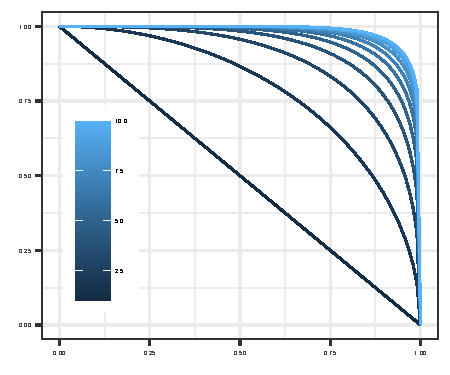
\includegraphics{images/p_sphere}
%    \caption{Unit hyperspheres established on $\mathcal{L}_p$, for $p = 1,\ldots,10$, for two dimensions.\label{fig:psphere}}
%\end{figure}

Consider a vector $\bm{s} \in {\mathbb R}^d$, and let the $\mathcal{L}_p$-norm be defined as
  \begin{equation*}
    \lVert \bm{s} \rVert_p = \left({\textstyle\sum}_{\ell = 1}^d \lvert s_{\ell}\rvert^p\right)^{\frac{1}{p}},
  \end{equation*}
for $p>0$. The absolute and Euclidean norms are obtained for $p=1$ and $p=2$ respectively. 
The $\mathcal{L}_{\infty}$ norm can be obtained as a limit, 
  \begin{equation*}
    \lVert \bm{s} \rVert_{\infty}
      = \lim\limits_{p\to\infty} \lVert \bm{s} \rVert_p
      = \max_{\ell\in\lbrace1,\ldots,d\rbrace}s_{\ell}.
  \end{equation*}
To define an angular measure,  we are interested in the direction of
vectors in ${\mathbb R}_{+}^d$, thus, we project them onto
  \begin{equation*}
    \mathcal{S}_{p}^{d-1} = \left\lbrace \bm{s} : \bm{s} \in {\mathbb R}_{+}^{d}, \lVert \bm{s}\rVert_{p} = 1\right\rbrace,
  \end{equation*}
  the $\mathcal{L}_p$-norm unit hypersphere.
  Given $\bm{x}\in {\mathbb R}^d_+$ the projection onto $\mathcal{S}_{p}^{d-1}$ is given as
  $\bm{y} = \bm{x} / \lVert \bm{x}\rVert_p \in \mathcal{S}_{p}^{d-1}$.
  Observations on one hypersphere can be projected without loss of information onto another by
  dividing by the defining norm of the target hypersphere. In fact, letting 
  \begin{equation*}
    y_d = \left(1 - {\textstyle\sum}_{\ell = 1}^{d-1}y_{\ell}^p\right)^{\frac{1}{p}}.
  \end{equation*}
  the transformation
  \begin{equation}
    \label{eqn:pnormt}
    T(x_1,\ldots,x_d) = \left(\pnorm{\bm{x}}{p}, \frac{x_1}{\pnorm{\bm{x}}{p}},
                          \ldots , \frac{x_{d-1}}{\pnorm{\bm{x}}{p}}\right) = (r,y_1,\ldots,y_{d-1})
  \end{equation}
  is invertible with
  \begin{equation}
    \label{eqn:pnormtinv}
    T^{-1}\left(r,y_1,\ldots,y_{d-1}\right) =
      \left(ry_1,\ldots,ry_{d-1}, r\left(1 - {\textstyle\sum}_{\ell = 1}^{d-1}y_{\ell}^p\right)^{\frac{1}{p}}\right).
  \end{equation}
  The Jacobian of the transformation takes the form
  \begin{equation}
    \label{eqn:pnormjac}
    r^{d-1}\left[\left(1 - {\textstyle\sum}_{\ell = 1}^{d-1}y_{\ell}^p\right)^{\frac{1}{p}} +
        {\textstyle\sum}_{\ell = 1}^{d-1}y_{\ell}^p\left(1 - {\textstyle\sum}_{l=1}^{d-1} y_{\ell}^p\right)^{\frac{1}{p} - 1}\right].
  \end{equation}
  Equations (\ref{eqn:pnormt}) -- (\ref{eqn:pnormjac}) can be used to define a density on ${\mathbb R}^p_+$, and then obtain a density on $\mathcal{S}_{p}^{d-1}$, for any finite $p>0$. Unfortunately in the limit, when $p\rightarrow +\infty$, the transformation is not differentiable. Thus, even though the projected distribution on $\mathcal{S}_\infty^{d-1}$ is defined, there is no corresponding density.
  
% EOF
